% The second eigenvalue of random regular graphs: notes to accompany slides.tex
% Compile from this folder with:  latexmk -pdf report.tex   (or pdflatex report.tex, twice)
\documentclass[11pt,letterpaper]{article}

\usepackage[T1]{fontenc}
\usepackage[utf8]{inputenc}
\usepackage{amsmath,amsthm,mathtools}
\usepackage{newpxtext}
\usepackage[smallerops]{newpxmath}
\usepackage[margin=1.15in]{geometry}
\usepackage{microtype}
\usepackage{booktabs,array}
\usepackage{enumitem}
\usepackage[font=small,labelfont=bf]{caption}
\usepackage{xcolor}
\usepackage{pgfplots}
\usepgfplotslibrary{groupplots}
\pgfplotsset{compat=1.16}
\usepackage[colorlinks=true,linkcolor=ink,citecolor=ink,urlcolor=ink]{hyperref}

\definecolor{ink}{HTML}{1B2A41}
\definecolor{accent}{HTML}{A23B1E}
\definecolor{barfill}{HTML}{C9D3DF}

% ---------- figure sizes ----------
\newcommand{\specw}{5.9cm}
\newcommand{\spech}{4.6cm}
\newcommand{\specsep}{0.5cm}
\newcommand{\nbw}{7.4cm}
\newcommand{\dyckunit}{5.2mm}
\newcommand{\shapeunit}{6.2mm}
\newcommand{\shapesep}{4.6cm}
\newcommand{\tangleunit}{7mm}
\newcommand{\dumbunit}{5mm}
\newcommand{\liftunit}{8mm}

% ---------- theorem environments ----------
\newtheorem{theorem}{Theorem}
\newtheorem{proposition}[theorem]{Proposition}
\theoremstyle{definition}
\newtheorem{example}[theorem]{Example}
\newtheorem{definition}[theorem]{Definition}
\theoremstyle{remark}
\newtheorem{remark}[theorem]{Remark}

% ---------- notation ----------
\DeclareMathOperator{\tr}{tr}
\newcommand{\edge}{2\sqrt{d-1}}
\newcommand{\eps}{\varepsilon}
\newcommand{\E}{\mathbb{E}}
\newcommand{\one}{\mathbf{1}}
\newcolumntype{L}[1]{>{\raggedright\arraybackslash}p{#1}}

\setlist{itemsep=2pt, topsep=4pt}

\begin{document}

\begin{center}
  {\LARGE\bfseries The second eigenvalue of random regular graphs\par}
  \vspace{6pt}
  {\large Notes on the Alon--Boppana bound, Friedman's theorem and the trace method\par}
\end{center}
\vspace{10pt}

\begin{abstract}
\noindent
A random $d$-regular graph has all of its non-trivial adjacency eigenvalues in the interval
$[-\edge-\eps,\ \edge+\eps]$ with high probability, and no large $d$-regular graph can do
better. These notes explain why $\edge$ is the barrier, why it is hard to prove that random
graphs reach it, and how the known proofs get around the difficulty. The emphasis is on
motivation and on the shape of the arguments; proofs are sketched, not given in full.
\end{abstract}

\section{Graphs as matrices}

Let $G$ be a graph on $n$ vertices with adjacency matrix $A$. Since $A$ is real and symmetric it
has real eigenvalues $\lambda_1\ge\lambda_2\ge\dots\ge\lambda_n$ and an orthonormal basis of
eigenvectors. The link between these eigenvalues and the combinatorics of $G$ is that powers of
$A$ count walks: the entry $(A^k)_{ij}$ is the number of walks of length $k$ from $i$ to $j$, where
a walk may repeat vertices and edges. Taking the trace gives the identity on which everything
below rests,
\begin{equation}\label{eq:trace}
  \tr(A^k)\;=\;\sum_{i=1}^{n}\lambda_i^{k}\;=\;\#\{\text{closed walks of length }k\text{ in }G\}.
\end{equation}

\begin{example}
The triangle has eigenvalues $2,-1,-1$. Formula \eqref{eq:trace} gives $2^3+(-1)^3+(-1)^3=6$
closed walks of length~$3$: three starting vertices and two directions.
\end{example}

Suppose now that $G$ is $d$-regular. Every row of $A$ sums to $d$, so the constant vector $\one$ is
an eigenvector with eigenvalue $d$. No eigenvalue exceeds $d$ in absolute value, since the number
of walks of length $k$ from any vertex is exactly $d^k$. Thus $\lambda_1=d$; this eigenvalue is
called \emph{trivial}, as is $-d$ when $G$ is bipartite. The subject of these notes is the size of
all the other eigenvalues, and we write
\[
  \mu(G)\;=\;\max\{|\lambda_i| : |\lambda_i|<d\}.
\]

\section{The spectral gap and expansion}

The quantity $d-\lambda_2$ is called the \emph{spectral gap}. It measures how far $G$ is from
being disconnected, and the reason is the following identity, valid for every vector $x$ indexed
by the vertices of a $d$-regular graph:
\begin{equation}\label{eq:dirichlet}
  d\,\lVert x\rVert^2-x^{\mathsf T}Ax\;=\;\sum_{\{u,v\}\in E}(x_u-x_v)^2 .
\end{equation}
The right-hand side measures how much $x$ varies across edges. Two consequences are immediate.
First, if $Ax=dx$ then the left side vanishes, so $x$ is constant on every connected component:
the multiplicity of the eigenvalue $d$ is the number of components. Second, since $\lambda_2$ is
the maximum of the Rayleigh quotient $x^{\mathsf T}Ax/\lVert x\rVert^2$ over $x\perp\one$,
\begin{equation}\label{eq:gap}
  d-\lambda_2\;=\;\min_{x\perp\one}\ \frac{\sum_{\{u,v\}\in E}(x_u-x_v)^2}{\sum_u x_u^2}.
\end{equation}
The gap is small exactly when some vector that sums to zero barely changes across any edge.

\begin{example}[A dumbbell]
Take two dense clusters of $n/2$ vertices each, joined by a single edge
(Figure~\ref{fig:dumbbell}). Let $x$ be $+1$ on one cluster and $-1$ on the other. Only the
joining edge contributes to the numerator of \eqref{eq:gap}, giving $4$, while the denominator is
$n$. Hence $d-\lambda_2\le 4/n$.
\end{example}

\begin{figure}[ht]
  \centering
  % Two dense clusters joined by a single edge.
% Requires: \dumbunit (unit length), colours ink, accent and barfill.
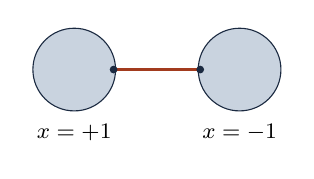
\begin{tikzpicture}[x=\dumbunit, y=\dumbunit]
  \draw[accent, thick] (-1.1,0) -- (1.1,0);
  \foreach \s/\lab in {-1/{+1}, 1/{-1}} {
    \fill[barfill] (2.1*\s,0) circle (1.05);
    \draw[ink] (2.1*\s,0) circle (1.05);
    \node[font=\footnotesize, anchor=north] at (2.1*\s,-1.15) {$x=\lab$};
  }
  \fill[ink] (-1.1,0) circle (1.4pt) (1.1,0) circle (1.4pt);
\end{tikzpicture}

  \caption{A dumbbell: one edge between two clusters forces a spectral gap of at most $4/n$.}
  \label{fig:dumbbell}
\end{figure}

The dumbbell argument works for any set of vertices, and it has a converse. Define the
\emph{edge expansion}
\[
  h(G)\;=\;\min_{0<|S|\le n/2}\ \frac{e(S,\bar S)}{|S|},
\]
where $e(S,\bar S)$ is the number of edges leaving $S$.

\begin{theorem}[Cheeger's inequality]\label{thm:cheeger}
For every $d$-regular graph $G$,
\[
  \frac{h(G)^2}{2d}\;\le\;d-\lambda_2\;\le\;2\,h(G).
\]
\end{theorem}

The upper bound is the dumbbell argument applied to an optimal set $S$. For the lower bound one
starts from a vector $x$ with small Rayleigh quotient in \eqref{eq:gap}, orders the vertices by
the value of $x$, and cuts at a well-chosen threshold; an edge crosses the cut only if the
threshold falls between its two values, which is rare when $x$ varies little across edges.

A family of $d$-regular graphs with $n\to\infty$ is an \emph{expander family} if $h$ stays above
a positive constant, or equivalently, by Theorem~\ref{thm:cheeger}, if the spectral gap does.
Expanders are sparse and yet have no bottleneck. The complete graph has no bottleneck but is not
sparse; the cycle and the complete binary tree are sparse but have $h$ of order $1/n$. Once the
gap is known to certify expansion, the natural question is how large it can be.

\section{The barrier \texorpdfstring{$\edge$}{2 sqrt(d-1)}}

The answer comes from the infinite $d$-regular tree $T_d$.

\paragraph{Closed walks in the tree.}
A closed walk of length $2k$ in a tree takes $k$ steps away from its starting vertex and $k$
steps back. It is determined by two choices (Figure~\ref{fig:dyck}). The first is the pattern of
away and back steps, which may never have more back steps than away steps so far; the number of
such patterns is the Catalan number $C_k\sim 4^k/(\sqrt{\pi}\,k^{3/2})$. The second is the branch
taken at each step away, for which there are at least $d-1$ choices. Each step back is forced,
because a vertex of a tree has a unique neighbour closer to the start. Up to polynomial factors
the number of closed walks of length $2k$ from a given vertex is therefore
\[
  4^k\,(d-1)^k\;=\;\bigl(\edge\bigr)^{2k}.
\]
The factor $2$ is the entropy of when to turn around; the factor $\sqrt{d-1}$ is the choice of
where to go, square-rooted because only half the steps are free.

\begin{figure}[ht]
  \centering
  % Distance from the starting vertex along a closed walk of length 12 in a tree.
% Requires: \dyckunit (length of one step), colours ink and accent.
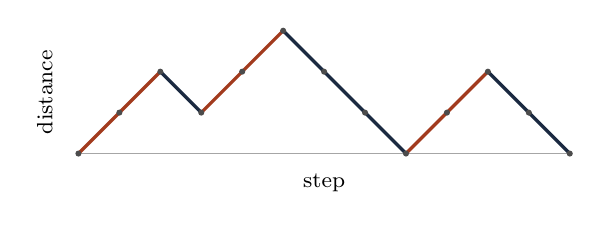
\begin{tikzpicture}[x=\dyckunit, y=\dyckunit, line cap=round, line join=round]
  \draw[black!35] (0,0) -- (12,0);
  \foreach \x/\y/\xx/\yy in {0/0/1/1, 1/1/2/2, 3/1/4/2, 4/2/5/3, 8/0/9/1, 9/1/10/2}
    \draw[accent, very thick] (\x,\y) -- (\xx,\yy);
  \foreach \x/\y/\xx/\yy in {2/2/3/1, 5/3/6/2, 6/2/7/1, 7/1/8/0, 10/2/11/1, 11/1/12/0}
    \draw[ink, very thick] (\x,\y) -- (\xx,\yy);
  \foreach \x/\y in {0/0,1/1,2/2,3/1,4/2,5/3,6/2,7/1,8/0,9/1,10/2,11/1,12/0}
    \fill[black!70] (\x,\y) circle (1.1pt);
  \node[font=\footnotesize, anchor=north] at (6,-0.25) {step};
  \node[font=\footnotesize, rotate=90, anchor=south] at (-0.4,1.5) {distance};
\end{tikzpicture}

  \caption{Distance from the starting vertex along a closed walk of length $12$ in a tree. Steps
  away (red) each have at least $d-1$ continuations; steps back (blue) are forced.}
  \label{fig:dyck}
\end{figure}

\begin{theorem}[Alon--Boppana]\label{thm:ab}
Every $d$-regular graph $G$ on $n$ vertices satisfies $\lambda_2(G)\ge\edge-o_n(1)$.
\end{theorem}

\begin{proof}[Sketch for $\mu(G)$]
Fix a vertex of $G$ and unroll $G$ from it into $T_d$, never identifying vertices reached by
different routes. This is the universal covering map $T_d\to G$. Every closed walk in the tree
projects to a closed walk in $G$, and distinct tree walks project to distinct walks; cycles in
$G$ only add further closed walks. By \eqref{eq:trace}, with $\rho=\edge$,
\[
  d^{2k}+(n-1)\,\mu^{2k}\;\ge\;\tr(A^{2k})\;\ge\;n\,C_k\,(d-1)^k\;\approx\;n\,\rho^{2k}\,k^{-3/2}.
\]
If $k$ is a sufficiently small multiple of $\log n$ then $d^{2k}$ is negligible beside
$n\rho^{2k}$, and taking $2k$-th roots gives $\mu\ge\rho-o(1)$. A refinement of the argument,
using test vectors supported on balls, gives the statement for $\lambda_2$ itself.
\end{proof}

Two features of the argument matter later. It applies to \emph{every} $d$-regular graph, including
graphs full of short cycles: the tree is the minimum. And it only works for $k=O(\log n)$; for
larger $k$ the single trivial eigenvalue swamps the count.

\begin{definition}
A $d$-regular graph is \emph{Ramanujan} if $\mu(G)\le\edge$.
\end{definition}

\section{Friedman's theorem and the trace method}

\begin{theorem}[Friedman \cite{F}; conjectured by Alon]\label{thm:friedman}
Fix $d\ge 3$ and $\eps>0$, and let $G$ be a uniformly random $d$-regular graph on $n$ vertices.
Then
\[
  \Pr\Bigl[\max\bigl(\lambda_2(G),\,|\lambda_n(G)|\bigr)\ge\edge+\eps\Bigr]\longrightarrow 0
  \qquad\text{as } n\to\infty .
\]
\end{theorem}

So almost every regular graph is almost Ramanujan. The bulk of the spectrum of a random regular
graph converges to the Kesten--McKay law, the spectral measure of $T_d$, which has density
\[
  \frac{d\,\sqrt{4(d-1)-x^2}}{2\pi\,(d^2-x^2)}\qquad\text{on } [-\edge,\ \edge];
\]
see Figure~\ref{fig:spectrum}. Eigenvalues near the edge of this interval are therefore expected.
The content of Theorem~\ref{thm:friedman} is that no eigenvalue lies outside it.

\begin{figure}[ht]
  \centering
  % Eigenvalue histograms of random d-regular graphs against the Kesten--McKay density.
% Requires: \specw, \spech (panel size), \specsep (gap), colours barfill and accent.
% The horizontal variable is t = lambda / (2 sqrt(d-1)), so the bulk is [-1, 1] in every panel.
\begin{tikzpicture}
\begin{groupplot}[
  group style={group size=3 by 1, horizontal sep=\specsep},
  width=\specw, height=\spech,
  xmin=-1.18, xmax=1.18, ymin=0, ymax=0.80,
  axis x line*=bottom, axis y line=none,
  xtick={-1,1}, tick align=outside, tick style={black!60},
  x axis line style={black!60},
  title style={font=\small, yshift=-1ex},
  ticklabel style={font=\footnotesize},
  clip=false,
]
\nextgroupplot[title={$d=3$}, xticklabels={$-2\sqrt{2}$, $2\sqrt{2}$}]
  \addplot[ybar, bar width=0.05, draw=white, line width=0.2pt, fill=barfill] table {data/hist_d3.dat};
  \addplot[accent, thick, domain=-1:1, samples=241]
    {2.828427*3*sqrt(max(0, 8 - (2.828427*x)^2)) / (2*pi*(9 - (2.828427*x)^2))};
\nextgroupplot[title={$d=6$}, xticklabels={$-2\sqrt{5}$, $2\sqrt{5}$}]
  \addplot[ybar, bar width=0.05, draw=white, line width=0.2pt, fill=barfill] table {data/hist_d6.dat};
  \addplot[accent, thick, domain=-1:1, samples=241]
    {4.472136*6*sqrt(max(0, 20 - (4.472136*x)^2)) / (2*pi*(36 - (4.472136*x)^2))};
\nextgroupplot[title={$d=16$}, xticklabels={$-2\sqrt{15}$, $2\sqrt{15}$}]
  \addplot[ybar, bar width=0.05, draw=white, line width=0.2pt, fill=barfill] table {data/hist_d16.dat};
  \addplot[accent, thick, domain=-1:1, samples=241]
    {7.745967*16*sqrt(max(0, 60 - (7.745967*x)^2)) / (2*pi*(256 - (7.745967*x)^2))};
\end{groupplot}
\end{tikzpicture}

  \caption{Non-trivial eigenvalues of one random $d$-regular graph on $2000$ vertices (bars),
  against the Kesten--McKay density (curve). The horizontal axis is rescaled so that the bulk
  edges $\pm\edge$ coincide across panels.}
  \label{fig:spectrum}
\end{figure}

\paragraph{Why long walks are needed.}
The trace is a sum over all eigenvalues, but the theorem concerns the largest. Suppose one could
show that $\sum_{i\ge2}\lambda_i^{2k}\le n(\rho+\eps)^{2k}$. Then
\begin{equation}\label{eq:amplifier}
  \mu^{2k}\;\le\;\sum_{i\ge 2}\lambda_i^{2k}\;\le\;n\,(\rho+\eps)^{2k}
  \qquad\Longrightarrow\qquad
  \mu\;\le\;n^{1/2k}\,(\rho+\eps),
\end{equation}
and the factor $n^{1/2k}$ tends to $1$ only if $k\gg\log n$. With $k$ of order $\log n$ it is a
constant, which is why the first results of this kind were off by a constant factor. Raising to
a high power acts as an amplifier: it lets one eigenvalue outweigh $n$ others.

This is the reverse of the situation in Theorem~\ref{thm:ab}. There, $k\asymp\log n$ sufficed,
and walks of that length are shorter than the diameter and see only the tree. For the upper bound
one needs $k\gg\log n$: the walks wrap around the graph many times, and must be counted to within
a factor $(1+\eps)^{2k}$.

\paragraph{The trivial eigenvalue.}
The term $d^{2k}$ must be removed exactly. This is possible because its eigenvector is known: the
matrix $A-\tfrac dn J$, where $J$ is the all-ones matrix, has the same eigenvalues as $A$ except
that $d$ is replaced by $0$.

\section{Tangles}

\paragraph{Counting by shape.}
For a random graph one computes $\E\tr(A^{2k})$ as a sum, over all potential closed walks, of the
probability that the walk is present. Walks are grouped by the \emph{shape} they trace, that is,
the subgraph formed by the distinct vertices and edges visited. A shape with $v$ vertices and
$e$ edges can be placed in about $n^v$ ways, and each placement is present with probability of
order $n^{-e}$, so
\begin{equation}\label{eq:shape}
  \E\bigl[\#\text{copies of the shape}\bigr]\;\asymp\;n^{\,v-e}.
\end{equation}
Each additional independent cycle costs a factor of $n$ (Figure~\ref{fig:shapes}). Tree-shaped
walks therefore dominate, contributing about $n\rho^{2k}$, which is why the spectrum of a random
graph resembles that of the tree. The random model enters the proof only through
\eqref{eq:shape}.

\begin{figure}[ht]
  \centering
  % Three shapes a closed walk can trace: a tree, a cycle, and two cycles sharing a vertex.
% Requires: \shapeunit (unit length), \shapesep (gap between shapes), colours ink and accent.
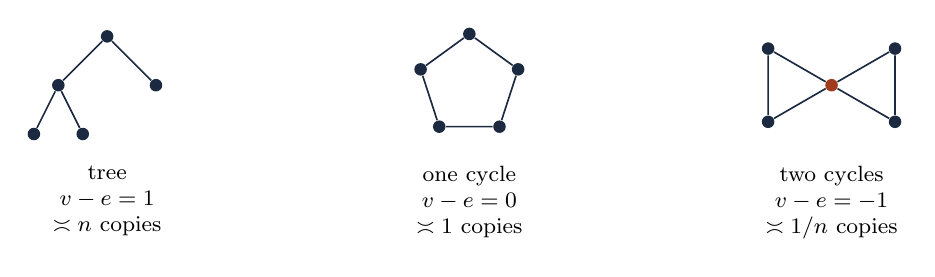
\begin{tikzpicture}[x=\shapeunit, y=\shapeunit,
    v/.style={circle, fill=ink, inner sep=1.6pt}, e/.style={ink, semithick}]
  % tree: v = 5, e = 4
  \begin{scope}[yshift={-1*\shapeunit}]
    \node[v] (a) at (0,2) {}; \node[v] (b) at (-1,1) {}; \node[v] (c) at (1,1) {};
    \node[v] (d) at (-1.5,0) {}; \node[v] (f) at (-0.5,0) {};
    \draw[e] (a)--(b) (a)--(c) (b)--(d) (b)--(f);
    \node[font=\footnotesize, align=center, anchor=north] at (0,-0.45) {tree\\ $v-e=1$\\ $\asymp n$ copies};
  \end{scope}
  % cycle: v = 5, e = 5
  \begin{scope}[xshift=\shapesep]
    \foreach \i in {0,...,4} \node[v] (p\i) at ({90+72*\i}:1.05) {};
    \draw[e] (p0)--(p1)--(p2)--(p3)--(p4)--(p0);
    \node[font=\footnotesize, align=center, anchor=north] at (0,-1.45) {one cycle\\ $v-e=0$\\ $\asymp 1$ copies};
  \end{scope}
  % two triangles sharing a vertex: v = 5, e = 6
  \begin{scope}[xshift={2*\shapesep}]
    \node[v, fill=accent] (o) at (0,0) {};
    \node[v] (l1) at (-1.3,0.75) {}; \node[v] (l2) at (-1.3,-0.75) {};
    \node[v] (r1) at (1.3,0.75) {};  \node[v] (r2) at (1.3,-0.75) {};
    \draw[e] (o)--(l1)--(l2)--(o) (o)--(r1)--(r2)--(o);
    \node[font=\footnotesize, align=center, anchor=north] at (0,-1.45) {two cycles\\ $v-e=-1$\\ $\asymp 1/n$ copies};
  \end{scope}
\end{tikzpicture}

  \caption{Three shapes with five vertices and their expected number of copies in a random
  regular graph.}
  \label{fig:shapes}
\end{figure}

\paragraph{The obstruction.}
Let $S$ be a fixed graph with $v-e=-c<0$, so that it occurs in $G$ with probability of order
$n^{-c}$, and suppose its presence forces an eigenvalue $\lambda_S>\rho$. Its contribution to
$\E\sum_{i\ge2}\lambda_i^{2k}$ is at least of order $n^{-c}\lambda_S^{2k}$, which exceeds the
target $n\rho^{2k}$ as soon as $k$ is a large multiple of $\log n$. Polynomial rarity cannot
compensate for exponential amplification. Such subgraphs are called \emph{tangles}. They do not
contradict Theorem~\ref{thm:friedman}, which only asserts high probability; they show that no
bound on the expectation can prove it.

\begin{example}[A vertex with $m$ self-loops]\label{ex:loops}
In the permutation model studied in \cite{F}, a $d$-regular multigraph is built from $d/2$
independent uniform permutations. A given vertex carries $m$ self-loops with probability
$n^{-m}$, so some vertex does with probability of order $n^{1-m}$. Non-backtracking walks
recirculate at such a vertex at rate $h=2m-1$ per step. If $h>\sqrt{d-1}$, consider the vector
equal to $1$ at the vertex and to $h^{-t}$ at distance $t$ from it, truncated at a large radius.
It has bounded norm because the decay beats the branching, $(d-1)/h^2<1$, and its Rayleigh
quotient is close to $h+(d-1)/h$. Since it is supported on a bounded number of vertices, it is
nearly orthogonal to $\one$, and one obtains \cite[Theorem~2.11]{F}
\[
  \lambda_2\;\ge\;h+\frac{d-1}{h}-o(1)\;>\;\edge .
\]
The smallest admissible $m$ gives the most likely tangle of this kind, and its probability
determines the rate in Friedman's theorem: the bound holds with probability
$1-O(n^{-\tau})$, where $\tau=\lceil(\sqrt{d-1}+1)/2\rceil-1$, and this cannot be improved in
general.
\end{example}

\begin{figure}[ht]
  \centering
  % A vertex with m = 3 self-loops in a d-regular graph, with trees hanging below it.
% Requires: \tangleunit (unit length), colours ink and accent.
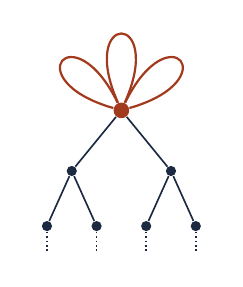
\begin{tikzpicture}[x=\tangleunit, y=\tangleunit,
    v/.style={circle, fill=ink, inner sep=1.3pt}, e/.style={ink, semithick}]
  % Explicit bounding box: the loops' control points would otherwise inflate it.
  \path[use as bounding box] (-1.7,-2.7) rectangle (1.7,1.5);
  \node[circle, fill=accent, inner sep=2pt] (o) at (0,0) {};
  \foreach \a in {40,90,140}
    \draw[accent, thick] (o) to[out=\a-24, in=\a+24, looseness=38] (o);
  \node[v] (a) at (-0.9,-1.1) {}; \node[v] (b) at (0.9,-1.1) {};
  \node[v] (a1) at (-1.35,-2.1) {}; \node[v] (a2) at (-0.45,-2.1) {};
  \node[v] (b1) at (0.45,-2.1) {};  \node[v] (b2) at (1.35,-2.1) {};
  \draw[e] (o)--(a) (o)--(b) (a)--(a1) (a)--(a2) (b)--(b1) (b)--(b2);
  \foreach \p in {a1,a2,b1,b2} \draw[e, densely dotted] (\p) -- ++(0,-0.5);
\end{tikzpicture}

  \caption{A vertex with three self-loops inside a $d$-regular graph. The surrounding
  neighbourhood is a tree.}
  \label{fig:tangle}
\end{figure}

\section{Selective traces}

The natural remedy is to condition on the absence of tangles. This fails for a technical reason:
\eqref{eq:shape} relies on the near-independence of edges, and conditioning on a global event
destroys it. The proofs instead change what is counted, not the probability space.

Define a modified trace that counts only those closed walks which trace no tangle. Friedman
calls his version the \emph{selective trace}; Bordenave \cite{B} counts \emph{tangle-free} paths.
Its expectation is taken over all graphs, with no conditioning, so the counting machinery still
applies. Two observations make this work:
\begin{itemize}
  \item on a tangle-free graph every walk qualifies, so the modified trace equals the true trace;
  \item on a graph containing a tangle the walks circulating inside it are not counted, so the
        rare event no longer contributes an exponentially large amount.
\end{itemize}
The theorem then follows from a union bound over the two ways to fail,
\[
  \Pr[\mu\text{ too large}]\;\le\;\Pr[\,G\text{ contains a tangle}\,]\;+\;\Pr[\,\text{modified trace is large}\,].
\]
The first term is small by \eqref{eq:shape}, the second by Markov's inequality applied to the
modified expectation.

What remains difficult is that ``traces no tangle'' is a non-local condition on a walk, which
makes the modified count much harder to evaluate than the plain one. Together with the exact
cancellation of the trivial eigenvalue, this accounts for the length of~\cite{F}.

\section{Non-backtracking walks}

The factor $2$ in $\edge$ comes entirely from backtracking. A walk is \emph{non-backtracking} if it
never traverses an edge and then immediately reverses it. From any vertex of a $d$-regular graph
there are exactly $d(d-1)^{k-1}$ such walks of length $k$, and a tree has no closed ones, so every
closed non-backtracking walk witnesses a cycle. Friedman's proof already counts these walks,
under the name \emph{irreducible}.

The \emph{non-backtracking matrix} $B$, also called the Hashimoto matrix, is indexed by the
$nd$ directed edges of $G$: the entry from $u\to v$ to $v\to w$ is $1$ if $w\ne u$ and $0$
otherwise. It is not symmetric, so its eigenvalues are complex.

\begin{theorem}[Ihara--Bass formula, $d$-regular case]\label{thm:ib}
Each eigenvalue $\lambda$ of $A$ gives rise to two eigenvalues $\mu$ of $B$, the roots of
\[
  \mu^2-\lambda\mu+(d-1)=0,\qquad\text{equivalently}\qquad\lambda=\mu+\frac{d-1}{\mu},
\]
and all remaining eigenvalues of $B$ are $\pm1$.
\end{theorem}

\begin{center}
\begin{tabular}{@{}ll@{}}
  \toprule
  Eigenvalue $\lambda$ of $A$ & Eigenvalues $\mu$ of $B$\\
  \midrule
  $\lambda=d$ & $d-1$ and $1$\\
  $|\lambda|<\edge$ & a complex-conjugate pair with $|\mu|=\sqrt{d-1}$\\
  $\lambda$ slightly above $\edge$ & two real values, one just outside the circle and one just inside\\
  \bottomrule
\end{tabular}
\end{center}

Consequently $G$ is Ramanujan exactly when every non-trivial eigenvalue of $B$ lies on the circle
of radius $\sqrt{d-1}$ (Figure~\ref{fig:nb}), and Friedman's theorem states that none has modulus
exceeding $\sqrt{d-1}+\eps$. The same relation explains Example~\ref{ex:loops}: a subgraph whose
own non-backtracking growth rate $h$ exceeds $\sqrt{d-1}$ lies outside the circle, and
$\lambda=h+(d-1)/h$ is the eigenvalue of $A$ it produces.

\begin{figure}[ht]
  \centering
  % Spectrum of the non-backtracking matrix of a random 4-regular graph on 150 vertices.
% Requires: \nbw (plot width), colours ink and accent.
\begin{tikzpicture}
\begin{axis}[
  width=\nbw, axis equal image,
  xmin=-2.3, xmax=3.6, ymin=-2.15, ymax=2.15,
  axis lines=middle, axis line style={black!45},
  xtick={-1,1,3}, ytick=\empty,
  ticklabel style={font=\footnotesize, fill=white, inner sep=1pt},
  tick style={black!45},
  xlabel={$\operatorname{Re}\mu$}, ylabel={$\operatorname{Im}\mu$},
  xlabel style={font=\footnotesize, at={(ticklabel* cs:1)}, anchor=west},
  ylabel style={font=\footnotesize, at={(ticklabel* cs:1)}, anchor=south},
  clip=false,
]
  \draw[accent, dashed] (axis cs:0,0) circle [radius=1.7320508];
  \addplot[only marks, mark=*, mark size=0.9pt, ink] table {data/nb_d4_n150.dat};
  \node[font=\footnotesize, accent, anchor=south west] at (axis cs:1.25,1.25) {$|\mu|=\sqrt{d-1}$};
  \node[font=\footnotesize, anchor=south] at (axis cs:3,0.15) {trivial};
\end{axis}
\end{tikzpicture}

  \caption{Eigenvalues of the non-backtracking matrix of a random $4$-regular graph on $150$
  vertices. The dashed circle has radius $\sqrt3$.}
  \label{fig:nb}
\end{figure}

\begin{remark}
Because the $\mu_i$ are complex, a bound on $\tr(B^k)=\sum_i\mu_i^k$ does not bound
$\max_i|\mu_i|$: the terms may cancel. Bordenave works instead with the operator norm of $B^k$
restricted to the complement of the trivial eigenvector.
\end{remark}

\section{Three proofs compared}

Table~\ref{tab:proofs} summarises three routes to Theorem~\ref{thm:friedman}. They trade
precision against length. Friedman and Kohler \cite{FK} extend the theorem to random covers of a
fixed base graph and simplify parts of the original method. Brito, Dumitriu and Harris \cite{BDH}
apply Bordenave's approach to random bipartite biregular graphs with degrees $d_1,d_2$, where the
bound becomes $\sqrt{d_1-1}+\sqrt{d_2-1}$. The polynomial method of Chen, Garza-Vargas, Tropp and
van Handel \cite{CGTV} avoids walk counting beyond the leading term altogether.

\begin{table}[ht]
\centering\small
\begin{tabular}{@{}L{0.17\textwidth}L{0.25\textwidth}L{0.24\textwidth}L{0.25\textwidth}@{}}
  \toprule
  & Friedman \cite{F} & Bordenave \cite{B} & Polynomial method \cite{CGTV}\\
  \midrule
  Object & Counts of closed non-backtracking walks & Operator norm of powers of $B$ & Expected traces of polynomials in $A$\\
    \addlinespace
  Tangles & Classified exactly by growth rate against $\sqrt{d-1}$ & Any neighbourhood containing two cycles & Not removed; visible in higher-order terms\\
    \addlinespace
  Trivial eigenvalue & Cancelled term by term in a $1/n$ expansion & Edge indicators centred by their mean & Trace is a rational function of $1/n$\\
    \addlinespace
  Failure probability & $O(n^{-\tau})$, optimal & $n^{-a}$ for any $a<1$ & Optimal in the permutation model\\
    \addlinespace
  Length & About 120 pages & About 20 pages & Short and general\\
  \bottomrule
\end{tabular}
\caption{Three proofs of Friedman's theorem.}
\label{tab:proofs}
\end{table}

\section{Beyond the literature}

This section records two things that lie at or beyond the edge of the published results above:
the definition of a graph lift, and a recovery problem for hidden partitions studied in an
unpublished manuscript. It is deliberately brief and states only what is understood at present.

\subsection{Graph lifts}

\begin{definition}
Let $H$ be a finite graph and $N\ge1$. An \emph{$N$-lift} of $H$ is a graph with vertex set
$V(H)\times[N]$, built as follows: for each edge $\{u,v\}$ of $H$ choose a permutation $\pi_{uv}$
of $[N]$, and join $(u,i)$ to $(v,\pi_{uv}(i))$ for every $i\in[N]$. The set $\{u\}\times[N]$ is
called the \emph{fibre} over $u$. In a \emph{random} $N$-lift the permutations are independent
and uniformly distributed.
\end{definition}

\begin{example}
The cube is a $2$-lift of the complete graph $K_4$ (Figure~\ref{fig:lift}). Label the vertices of
the cube by binary triples; the four fibres are the four pairs of antipodal vertices, and each
vertex has exactly one neighbour in each of the three other fibres.
\end{example}

\begin{figure}[ht]
  \centering
  % The cube as a 2-lift of K_4: each fibre is a pair of antipodal vertices.
% Requires: \liftunit (unit length), colours ink and accent.
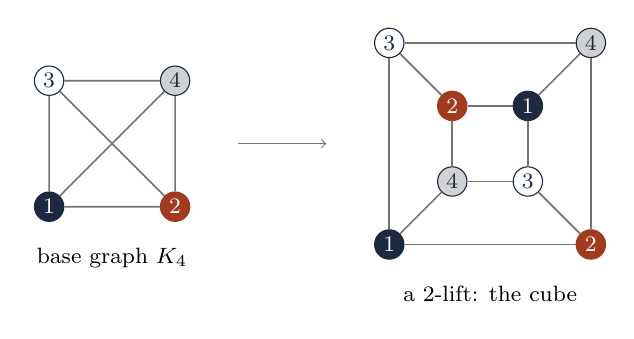
\begin{tikzpicture}[x=\liftunit, y=\liftunit,
    e/.style={black!55, semithick},
    f1/.style={circle, draw=ink, fill=ink, text=white, inner sep=1.4pt, font=\footnotesize},
    f2/.style={circle, draw=accent, fill=accent, text=white, inner sep=1.4pt, font=\footnotesize},
    f3/.style={circle, draw=ink, fill=white, text=ink, inner sep=1.4pt, font=\footnotesize},
    f4/.style={circle, draw=ink, fill=black!18, text=ink, inner sep=1.4pt, font=\footnotesize}]
  % base graph K_4
  \begin{scope}
    \node[f1] (a) at (0,0) {1}; \node[f2] (b) at (2,0) {2};
    \node[f4] (c) at (2,2) {4}; \node[f3] (d) at (0,2) {3};
    \draw[e] (a)--(b)--(c)--(d)--(a) (a)--(c) (b)--(d);
    \node[font=\footnotesize, anchor=north] at (1,-0.5) {base graph $K_4$};
  \end{scope}
  \draw[->, black!55] (3.0,1) -- (4.4,1);
  % the cube: vertices are binary triples, antipodal pairs form the fibres
  \begin{scope}[xshift={5.4*\liftunit}, yshift={-0.6*\liftunit}]
    \node[f1] (v000) at (0,0) {1};     \node[f2] (v100) at (3.2,0) {2};
    \node[f4] (v110) at (3.2,3.2) {4}; \node[f3] (v010) at (0,3.2) {3};
    \node[f4] (v001) at (1,1) {4};     \node[f3] (v101) at (2.2,1) {3};
    \node[f1] (v111) at (2.2,2.2) {1}; \node[f2] (v011) at (1,2.2) {2};
    \draw[e] (v000)--(v100)--(v110)--(v010)--(v000);
    \draw[e] (v001)--(v101)--(v111)--(v011)--(v001);
    \draw[e] (v000)--(v001) (v100)--(v101) (v110)--(v111) (v010)--(v011);
    \node[font=\footnotesize, anchor=north] at (1.6,-0.5) {a $2$-lift: the cube};
  \end{scope}
\end{tikzpicture}

  \caption{The cube as a $2$-lift of $K_4$. Vertices with the same label form a fibre.}
  \label{fig:lift}
\end{figure}

Two properties follow at once from the definition. A lift of a $d$-regular graph is $d$-regular.
And every vertex in the fibre over $u$ has exactly one neighbour in the fibre over each neighbour
of $u$, and none in any other fibre. Lifts connect to the earlier sections in two ways: the
permutation model of Example~\ref{ex:loops} is a random lift of a single vertex with $d/2$ loops,
and the extensions of Friedman's theorem in \cite{FK,B} concern random lifts of a fixed base
graph.

\subsection{Recovering a hidden partition}

\begin{definition}
A partition $V=V_1\sqcup\dots\sqcup V_k$ of the vertex set of a graph has \emph{exact neighbour
counts} $(b_{ij})$ if every vertex of $V_i$ has exactly $b_{ij}$ neighbours in $V_j$, for all
$i$ and $j$.
\end{definition}

For example, the fibres of any lift of a simple graph $H$ form such a partition, with $b_{uv}=1$
when $u$ and $v$ are adjacent in $H$ and $b_{uv}=0$ otherwise. A second example, not a lift, has
two classes in which every vertex has two neighbours in its own class and one in the other.

\paragraph{The problem.}
Fix the counts and plant a partition: choose the graph at random, uniformly subject to the
prescribed counts within and between classes, and then erase the labels. The task is to recover
the partition from the graph alone. The algorithm is given neither the counts nor the number of
classes, only upper bounds $K$ on the number of classes and $\Delta$ on the degrees.

\paragraph{Claimed results.}
The following statements are those of an unpublished manuscript, known to us through a
plain-language companion document. They have not been refereed, and they are reported here as
claims.
\begin{itemize}
  \item \emph{Scope.} The results hold under a condition on the counts which is satisfied whenever
  every vertex has the same degree $d\ge3$. In particular they cover random lifts of every fixed
  connected simple $d$-regular graph with $d\ge3$, with the fibres as the planted classes.
  Minimum degree three alone is not claimed to suffice.
  \item \emph{Listing.} There is an algorithm that lists every partition with exact neighbour
  counts and at most $K$ classes. Its output is always correct; its expected running time is
  $n^2(\log n)^{O(1)}$ and its expected memory is $n(\log n)^{O(1)}$, where $n$ is the number of
  vertices and the constants depend on $K$ and $\Delta$.
  \item \emph{Recovery.} With probability tending to one, every listed partition is obtained by
  merging planted classes, so the finest listed partition is the planted one up to renaming the
  classes.
  \item \emph{Ambiguity.} For two classes of size $N$ with counts ``two inside, one across'', the
  probability that a second valid partition exists is asymptotic to $4/N^2$, and the smallest
  possible average recovery error is asymptotic to $2/N^2$.
\end{itemize}

\paragraph{Method.}
The neighbour-count conditions are linear equations in the indicator vectors of the classes.
The algorithm solves them over a finite field, which describes a possibly large set of candidates
by a small basis, and then checks each candidate against the original integer counts. A candidate
that satisfies the equations only modulo a prime fails this check.

\paragraph{Relation to the rest of these notes.}
Spectral methods for finding hidden structure usually need the relevant eigenvalue to be
separated from the bulk, which is the kind of statement Friedman's theorem provides. The approach
above uses exact equations instead and assumes no eigenvalue gap. Its limits are correspondingly
strict: the number of classes and the degrees are fixed as $n$ grows, the counts must be exact,
and nothing is claimed for graphs perturbed by noise.

\section{Numerical illustrations}

The figures come from small simulations in the configuration model, which allows loops and
multiple edges. They are illustrations at a single size, not evidence for the theorems.

\paragraph{Extreme eigenvalues.}
Table~\ref{tab:extreme} lists the extreme non-trivial eigenvalues of the three graphs in
Figure~\ref{fig:spectrum}. All lie within $0.02$ of $\pm\edge$, on either side, as the $\eps$ in
Theorem~\ref{thm:friedman} allows.

\begin{table}[ht]
\centering\small
\begin{tabular}{@{}rrrr@{}}
  \toprule
  $d$ & $\edge$ & $\lambda_2$ & $\lambda_n$\\
  \midrule
  $3$ & $2.828$ & $2.824$ & $-2.830$\\
  $6$ & $4.472$ & $4.467$ & $-4.452$\\
  $16$ & $7.746$ & $7.749$ & $-7.727$\\
  \bottomrule
\end{tabular}
\caption{One random $d$-regular graph on $2000$ vertices for each $d$.}
\label{tab:extreme}
\end{table}

\paragraph{A planted tangle.}
For $d=8$ and $n=2000$, a random graph had $\lambda_2=5.251$, below $2\sqrt7\approx5.292$.
Planting three self-loops at one vertex, so that $h=5>\sqrt7$, gave $\lambda_2$ between $6.396$
and $6.398$ in five samples. Example~\ref{ex:loops} predicts $h+(d-1)/h=5+7/5=6.4$.

\paragraph{Non-backtracking spectrum.}
For the graph of Figure~\ref{fig:nb}, the matrix $B$ is $600\times600$. Its largest eigenvalue is
$3=d-1$ and the largest non-trivial modulus is $1.7321\approx\sqrt3$, so this sample is
Ramanujan.

\begin{thebibliography}{9}

\bibitem{F}
J.~Friedman.
\newblock A proof of Alon's second eigenvalue conjecture and related problems.
\newblock \emph{Mem.\ Amer.\ Math.\ Soc.}\ 195 (2008), no.~910.
\newblock \href{https://arxiv.org/abs/cs/0405020}{arXiv:cs/0405020}.

\bibitem{FK}
J.~Friedman and D.-E.~Kohler.
\newblock The relativized second eigenvalue conjecture of Alon.
\newblock Preprint, 2014. \href{https://arxiv.org/abs/1403.3462}{arXiv:1403.3462}.

\bibitem{B}
C.~Bordenave.
\newblock A new proof of Friedman's second eigenvalue theorem and its extension to random lifts.
\newblock \emph{Ann.\ Sci.\ \'Ec.\ Norm.\ Sup\'er.}\ 53 (2020).
\newblock \href{https://arxiv.org/abs/1502.04482}{arXiv:1502.04482}.

\bibitem{BDH}
G.~Brito, I.~Dumitriu and K.~D.~Harris.
\newblock Spectral gap in random bipartite biregular graphs and applications.
\newblock \emph{Combin.\ Probab.\ Comput.}\ 31 (2022).
\newblock \href{https://arxiv.org/abs/1804.07808}{arXiv:1804.07808}.

\bibitem{CGTV}
C.-F.~Chen, J.~Garza-Vargas, J.~A.~Tropp and R.~van Handel.
\newblock A new approach to strong convergence.
\newblock Preprint, 2024. \href{https://arxiv.org/abs/2405.16026}{arXiv:2405.16026}.

\end{thebibliography}

\end{document}
